\documentclass[12pt]{article}
\usepackage[margin=1in]{geometry}
\usepackage[svgnames]{xcolor}
\usepackage[utf8]{inputenc}
\usepackage{graphicx}
\usepackage{setspace}
\usepackage{hyperref}
\usepackage{scrextend}
\usepackage{nameref}
\usepackage{fancyhdr}
\usepackage{indentfirst}
\usepackage{amsmath}
\usepackage{amsfonts}
\usepackage{amssymb}
\usepackage{enumerate}
\usepackage{ragged2e}
\usepackage{marginnote}
\usepackage{float}
\usepackage{tcolorbox}
\usepackage{wrapfig}
\usepackage{lipsum}
\tcbuselibrary{skins}
\tcbuselibrary{breakable}
\usetikzlibrary{decorations.pathmorphing}
\doublespacing
\numberwithin{equation}{section}

\usetikzlibrary{decorations.pathmorphing}

\graphicspath{{/Users/richard/Documents/Ouvrages/Latex_Note/Figures/}}
% Def a global settings for box styles:
\tcbset{
style_pic/.style={tile,beamer,colback=Honeydew!50!white,colframe=LightGray},
style_eq/.style={beamer,breakable,colback=DarkGoldenrod!37},
style_theo/.style={breakable,beamer,frame style={left color=red!75!black,right color=blue!75!black},interior style={left color=LightCoral!35!Azure,right color=Azure!60!AliceBlue} ,fonttitle=\bfseries, opacityback=0.95, titlerule=2pt,},    
style_def/.style={beamer,breakable,enhanced,colback=Lavender!50,colframe=LightSteelBlue!70,colbacktitle=DarkSeaGreen!75!black,fonttitle=\bfseries,borderline north={3pt}{-1.5pt}{Navy!20!white,decoration={zigzag,amplitude=2pt},decorate},borderline south={3pt}{-1.5pt}{Navy!20!white,decoration={zigzag,amplitude=2pt},decorate},boxrule=0pt,sharp corners,toprule=1.25mm,bottomrule=1.25mm},
style_lemma/.style={beamer,breakable,colframe=FireBrick!55!Black,interior style={top color=LightSalmon!40!white,bottom color=MintCream!30!white},fonttitle=\bfseries},
style_coro/.style={beamer,breakable,colframe=Aqua!50!black,interior style={top color=LightBlue!70!,bottom color=MintCream},fonttitle=\bfseries},
style_proof/.style={beamer,breakable,title=Concise Summery,breakable,enhanced,skin=enhancedlast jigsaw,attach boxed title to top left={xshift=-4mm,yshift=-0.5mm}, fonttitle=\bfseries\sffamily,interior style={top color=MediumPurple!45!white,bottom color=DeepSkyBlue!15!white}, boxed title style={empty,arc=0pt,outer arc=0pt,boxrule=0pt}, underlay boxed title={ \fill[BlueViolet!85!White] (title.north west) -- (title.north east)-- +(\tcboxedtitleheight-1mm,-\tcboxedtitleheight+1mm)-- ([xshift=4mm,yshift=0.5mm]frame.north east) -- +(0mm,-1mm)-- (title.south west) -- cycle;\fill[Indigo] ([yshift=-0.5mm]frame.north west)-- +(-0.4,0)--+(0,-0.3)--cycle;
        \fill[Indigo] ([yshift=-0.5mm]frame.north east)-- +(0,-0.3) -- +(0.4,0) -- cycle; }}
}

% Def a box for picture:
\newtcbox[auto counter, number within=section]{\picbox}[2][]{style_pic,title=Figure \thetcbcounter:~#2,label=pic:\thetcbcounter,#1}
% Def new command:
\let\bb\mathbb
\newcommand{\tincludegraphics}[3][]{\center\picbox{#3}{\includegraphics[width=310pt,#1]{#2}}}
% Def theorem environment:
\newtcolorbox[auto counter,number within=section]{box_for_theo}[2][]{style_theo,title=Theorem \thetcbcounter:~#2,label=th:\thetcbcounter,#1}


\newenvironment{theo}[2][]{\begin{box_for_theo}[#1]{#2}}{\end{box_for_theo}}

% Def lemma environment:
\newtcolorbox[auto counter, number within=section]{box_for_lemma}[2][]{style_lemma,title=Lemma \thetcbcounter:~#2,label=le:\thetcbcounter,#1}

\newenvironment{lem}[2][]{\begin{box_for_lemma}[#1]{#2}}{\end{box_for_lemma}}

% Def corollary environment:
\newtcolorbox[auto counter, number within=section]{box_for_coro}[2][]{style_coro,title=Corollary \thetcbcounter:~#2,label=co:\thetcbcounter,#1}

\newenvironment{coro}[2][]{\begin{box_for_coro}[#1]{#2}}{\end{box_for_coro}}

% Def definition environment:
\newtcolorbox[auto counter,number within=section]{box_for_def}[2][]{style_def,title=Definition \thetcbcounter:~#2,label=def:\thetcbcounter,#1}

\newenvironment{defi}[2][]{\begin{box_for_def}[#1]{#2}}{\end{box_for_def}}

% Def proof environment:
\newtcolorbox{box_for_proof}{style_proof}

\newenvironment{proof}{\begin{box_for_proof}}{\end{box_for_proof}}

% Def Equation environment:
\newenvironment{eq}[2][]{\begin{equation}\tcboxmath[style_eq,label=eq:#1]{#2}}{\end{equation}}


% header and footer:

\pagestyle{fancy}
\rhead{\textbf{\thepage}}
\chead{}
\lhead{}
\lfoot{}
\cfoot{}
\rfoot{}
\renewcommand{\headrulewidth}{0pt}

% customized command:
\let\bb\mathbb
\newcommand{\suppose}{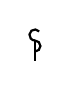
\begin{tikzpicture}[scale=0.35,thick]

\draw (1.55mm,-0.7mm)arc (40:270:2mm);
\draw (-0mm,-8mm)arc (270:450:2mm);
\draw (0,-4mm)--(0,-11.5mm);
\end{tikzpicture} }

\begin{document}

\begin{titlepage}
    \hspace{0pt}
    \vfill
    \begin{tcolorbox}[style_def]
    \begin{center}
        \rule{\textwidth}{1.5pt}\\[1mm]
        \LARGE{\textbf{Avila Project}}\\[3mm]
        \large{\textbf{possible questions regarding to the Avila project}}\\[1mm]
        \rule{\textwidth}{1.5pt}\\[1mm]
    \end{center}
    \end{tcolorbox}
    \vfill
    \begin{tcolorbox}[style_pic]
        \begin{center}
            \large{Author: \textbf{Richard Lu}}\\
            \large{Date:}\\
            \large{\today}
        \end{center}
    \end{tcolorbox}
\end{titlepage}


\section{Questions and Summery}

\begin{theo}[title=Question 1]{}
	What is the goal of the Project? Why this is called Avila project?
\end{theo}

\vspace{10mm}

\begin{proof}
	\begin{enumerate}
		\item Our aim is to learn and extract the features from the dataset in a more efficient and effective way. The general methods applied here are unsupervised deep learning which consists a multi-layer NN (Neural network). Hence, we wish  to construct a customized NN that eventually fulfill our goal.
		\item our project is called Avila which is named after `The Avila Bible case study'. It's a studied dataset with the task of Reliable writer identification in medieval manuscripts through page layout features.
	\end{enumerate}
	
\end{proof}

\vspace{10mm}

\begin{theo}[title=Question 2]{}
	More specific goals? What are the methods used in the exploration?
\end{theo}

\vspace{10mm}

\begin{proof}
	\begin{enumerate}
		\item In order to extract a more interpretable feature from the dataset. We focus on two important characteristics of the feature. The first one is that we intend to find the most influential (most) weighted feature among all. The second is that we wish to find the most concise feature representation to the dataset, which means to search the compressed feature with minimal dimension and minimal data loss.
		\item As for searching the compressed feature, there are several ways to do it. We compare the results of applying different techniques of data compression (PCA, SVD, AE-NN) to our datasets and find that the Auto-encoder(AE), as a NN compression method, works the best for our specific dataset and thus use it as a base model to derive and construct our own customized AE model (C-AENet)
		\item For the other goal, we wish to extract the most influential feature among the important features from the dataset. This process can be done by the famouse SE Network or SE module (Squeeze and excitation module). And based on this SE module, we also create a customized SE model called C-SENet to better accommodate our dataset.
		\item Lastly, it is also interesting to take a step further and make a combined model with both C-AE module and C-SE module. Thus we create a customized AESE model (C-AESENet) by sequentially merge the AE module and SE module into the normal NN.
	\end{enumerate}
	
\end{proof}

\vspace{10mm}

\begin{theo}[title=Question 3]{}
	Does the result for each model look promising? Some final conclusion? 
\end{theo}

\vspace{10mm}
	
\begin{proof}
	\begin{enumerate}
		\item The results we got from the experiments are pretty promising and are almost exactly as we expected.
		\item C-AENet has almost the same accuracy with the base model which means it did really well in feature compression and could potentially compress the core feature data without losing anything. 
		\item C-SENet has the highest accuracy among all the model, which means it has the ability to capture the essence of the data and using this weighted feature to label the test group fairly well.
		\item C-AESENet has the accuracy between C-AENet and C-SENet. Hence it could in theory not only capture the weighted feature among data but also compress this feature data with minimal data loss.
		\item Experimental results on the Avila dataset show that the model we provided (with both C-AENet and C-SENet) has great potential to provide a robust feature representation for data classification and can be widely adopted in most classification tasks.
	\end{enumerate}
\end{proof}

\end{document}













